%%% fs-seim-typical - Typical solutions

\label {fs-typical}

There are two most common methods that are used to implement order-sensitive operators: in-order processing (IOP) \cite{Arasu:2006:CCQ:1146461.1146463, Cranor:2003:GSD:872757.872838, hammad2004optimizing} and out-of-order processing (OOP) \cite{Li:2008:OPN:1453856.1453890}.

\subsection{In-order processing}
According to IOP approach, each operation must enforce the total order on output elements that can be violated due to asynchronous nature of execution. Buffering is usually used to fulfill this requirement. Figure~\ref{iop} shows the union operation that combines multiple streams into the single one. Both input streams are ordered, as predecessors must meet ordering constraint. Nevertheless, if there is arrival time skew between input streams, the union must buffer the earlier stream to produce ordered output. It is known that IOP is memory demanding and has unpredictable latencies and limited scalability \cite{Li:2008:OPN:1453856.1453890}.

\begin{figure}[htbp]
  \centering
  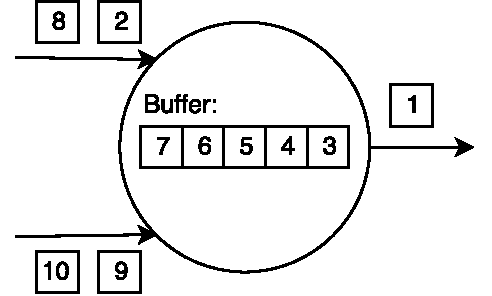
\includegraphics[width=0.30\textwidth]{pics/iop}
  \caption{IOP union operation. Due to delay of the upper stream operation must buffer elements}
  \label {iop}
\end{figure}

\subsection{Out-of-order processing}
OOP is an approach that does not require order maintenance if it is not needed. In the case of ordering requirements, OOP buffers input items until a special condition is satisfied. This condition is supported by progress indicators such as punctuations \cite{Tucker:2003:EPS:776752.776780}, low watermarks \cite{Akidau:2013:MFS:2536222.2536229}, or heartbeats \cite{Srivastava:2004:FTM:1055558.1055596}. They go through the stream as ordinal items, but do not trigger business-logic of the operations. Each progress indicator carries meta-information and promises that there are no any elements with lesser meta-information. Therefore, indicators must be monotonic, but data items between two consecutive indicators can be arbitrarily reordered. Data sources periodically yield them.

A timed window operation can be mentioned as an example of OOP approach. A window operation buffers partial results until a progress indicator arrives. After that, the window flushes corresponding buffers and propagates the indicator to the next operation down the stream.

OOP addresses the downsides of the IOP, but it has flaws too. Even if the input stream is totally ordered, the operation must wait for the progress indicator. Figure~\ref{oop} illustrates such case. Bottom window is complete but must be blocked until the indicator for the item 11 arrives. Another issue of OOP is that periodical flushes can result in load bursts and an increase in latency. 

\begin{figure}[htbp]
  \centering
  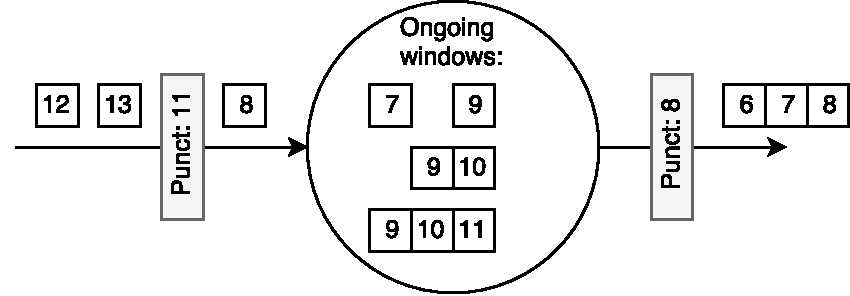
\includegraphics[width=0.48\textwidth]{pics/oop}
  \caption{OOP sliding window, range=3, slide=1. Operation must block lower window until next punctuation arrival }
  \label {oop}
\end{figure}
